\documentclass[12pt, twoside, a4paper]{report}

\usepackage{amsmath}
\usepackage{dsfont}
\usepackage[toc, page]{appendix}
\usepackage{graphicx}
\usepackage[sort&compress]{natbib}
\usepackage{subcaption}
\usepackage[nottoc]{tocbibind}

% Location of the graphics files
\graphicspath{{figures/}}
% Set line spacing
\linespread{1.5}

\begin{document}

\title{Real-time Pedestrian Modelling: Implementing the Ensemble Kalman Filter
for an Agent-Based Model}
\author{Keiran Suchak --- 200888140}
\maketitle

\chapter*{\centering Abstract}
\addcontentsline{toc}{chapter}{Abstract}

This is the abstract.

\tableofcontents
\listoffigures
\listoftables

%\chapter*{Notes}

%\begin{itemize}
    %\item What is data assimilation?
    %\item What is the Ensemble Kalman Filter?
    %\item What are Agent-Based Models?
    %\item How do people model pedestrians?
    %\item What happens when an agent in one of the ensemble member models tries
        %to leave the station early? Because we're only doing state estimation
        %(meaning just the agent coordinates), the agent won't get reactivated.
    %\item Errors should converge on something relating to twice the exit
        %distance.
    %\item Signposting at the beginning of each chapter
    %\item Don't need to review calibration too much
    %\item Don't need to talk about different types of enkf's too much
    %\item Don't need to talk about DA with CA too much
%\end{itemize}

%\section*{Structure}

%\begin{itemize}
    %\item What is the problem?
    %\item Why should people care?
    %\item What has been done in the past to try to solve the problem?
    %\item What are we doing to solve the problem? How is this different?
    %\item How well does our attempt work? How does this compare to others?
%\end{itemize}

\include{chapters/introduction}

\chapter{Literature Review}\label{ch:lit_rev}

%\begin{itemize}
    %\item DATA ASSIMILATION IN GENERAL
    %\item HOW THIS RELATES TO CALIBRATION
%\end{itemize}

As touched upon in Chapter \ref{ch:intro}, the process of developing an
agent-based model typically involves some form of model calibration.
Model calibration is the procedure of fine-tuning the model that we are using
such that it best fits the particular situation that we are seeking to model
\citep{crooks2012introduction}.
There are a large number of different manners in which we can calibrate
agent-based models \citep{thiele2014facilitating}.
These approaches typically involve making use of real-world data to estimate the
parameters and initial state of the model; this is, however, undertaken once
prior to running the model.

In some situations, we aim to simulate events in real-time (or close to
real-time).
In such situations, we are often able to observe the evolution of
the real-world system which we seek to model and consequently may wish to use
this information to recalibrate the model.
This would, however, require that we stop the simulation, undertake calibration,
and restart the model.
We therefore seek an approach that allows us to incorporate observations of the
system whilst simulating the system --- data assimilation.

This Chapter will therefore seek to provide a basic overview of data
assimilation, along with some coverage of the attempts that have been made to
implement such techniques to agent-based models that simulate urban systems.

\section{Data Assimilation}\label{sec:method:da}

\begin{itemize}
    \item Origins of filtering with Wiener filter, 1950. Only applies for
        stationary signals.
    \item Kalman-Bucy 1961
    \item Stratonovich 1968
    \item Jazwinski 1970
    \item 
\end{itemize}

The process of data assimilation involves making use of observations along with
prior knowledge (which, in our case, is encoded in a model) to produce
increasingly accurate estimates of variables of interest.
Such a process can be achieved through a Bayesian filtering approach
\citep{jazwinski1970mathematics, bar2004estimation}.

Under such a framework, the updating of the model state is undertaken on the
basis of Bayes Rule (for which a derivation is provided in Appendix
\ref{ch:bayes}):
\begin{equation}
    P(A|B) = \frac{P(B|A) P(A)}{P(B)}
\end{equation}
Bayes Rule is made up of four components:
\begin{enumerate}
    \item $P \left( A \right)$: The probability of $A$, known as the
        \textbf{Prior}.
    \item $P \left( A|B \right)$: The probability of $A$ given $B$, known as the
        \textbf{Posterior}.
    \item $P \left( B|A \right)$: The probability of $B$ given $A$, known as the
        \textbf{Likelihood}.
    \item $P \left( B \right)$: The probability of $B$, known as the
        \textbf{Marginal Likelihood}.
\end{enumerate}
When applying this notation to the problem at hand, the components become:
\begin{enumerate}
    \item \textbf{Prior}, $P(\mathbf{x})$: The probability distribution
        representing the prior state of the model.
    \item \textbf{Posterior}, $P(\mathbf{x}|\mathbf{d})$: The probability
        distribution representing the updated state of the model in light of the
        observed data, that is to say the probability of the model state given
        the data.
    \item \textbf{Likelihood}, $P(\mathbf{d}|\mathbf{x})$: The probability
        distribution of the observed data given the model state.
    \item \textbf{Marginal Likelihood}, $P(\mathbf{d})$: The probability
        distribution representing the observed data.
\end{enumerate}
With the above notation, Bayes Rule becomes:
\begin{equation}
    P \left( \mathbf{x} | \mathbf{d} \right) =
       \frac{P \left( \mathbf{d} | \mathbf{x} \right)
             P \left( \mathbf{x} \right)}{P \left( \mathbf{d} \right)} 
\end{equation}
The aim of a data assimilation scheme therefore becomes to provide an update to
the  state in the form of the posterior, $P \left( \mathbf{x} | \mathbf{d}
\right)$, given new observations, $P \left( \mathbf{d} \right)$.

There exist a number of different schemes for tackling this problem which are
often divided into two groups:
\begin{enumerate}
    \item \textbf{Sequential}: What does this mean and some examples, Kalman
        Filter (and variations thereof), Particle Filter.
    \item \textbf{Variational}: What does this mean and some examples, 3D-VAR,
        4D-VAR.
\end{enumerate}

Of the work that currently exists wherein investigators attempt to apply data
assimilation schemes to agent-based models, most make use of sequential schemes. 

\section[Application of Data Assimilation to Agent-Based Models]{Application of Sequential Data Assimilation to Agent-Based
Models}\label{sec:lit_rev:da_abm}

%Agent-based simulation is useful for studying people's movement in smart
%environment.
%Existing agent-based simulations are typically used as offline tools that help
%system design.
%They are not dynamically data-driven because they do not utilise any real time
%sensor data of the environment.
%In this paper, we present a method that assimilates real time sensor data into
%an agent-based simulation model.
%The goal of data assimilation is to provide inference of people's occupancy
%information in the smart environment, and thus lead to more accurate simulation
%results.
%We use particle filters to carry out the data assimilation and present some
%experiment results, and discuss how to extend this work for more advanced data
%assimilation in agent-based simulation of smart environment.

%\begin{itemize}
    %\item Environment:
    %\item Data source: synthetic data generated by the model.
    %\item Type of data: Sensors report presence of agent at position.
    %\item Method: Particle filter
    %\item Experiments run: different routing types, different number of
        %particles, single agent, two agents (set up such that agents are less
        %likely to interact).
    %\item Findings:
%\end{itemize}

One of earliest pieces of work undertaken on the application of data
assimilation schemes to agent-based models of urban environments was by
\citet{wang2013data}.
In this work, they simulate a smart office environment with people in it --- a
scenario that is becoming increasingly common with the advent of the Internet of
Things.
The aim of the work was to make use of real-time data in conjunction with the
agent-based simulation to provide more accurate estimates of the occupancy of
the environment.
This was achieved using the Particle Filter method of data assimilation; the
method was chosen as it did not require the system to be Gaussian.
The particle filter method operates by holding an ensemble of realisations of
the simulation, each of which are evolved forward over time between
observations; when observations are received, the particle states are weighted
and the new state is obtained by sampling from these weighted particles.
The observations used were synthetic data generated by the agent-based model,
aiming to emulate motion sensors which would provide a binary response of
whether a person was present in a given location.

The work undertaken consisted of two experiments --- firstly simulating single
agent in the environment, then going on to simulate two agents in the same
environment.
In the case if the first experiment, the agent was simulated with two different
routing behaviours; for the first routing behaviour, the agent move forward
sequentially through a series of waypoints, whilst for the second routing
behaviour, the agent moves through a series of waypoints before turning back to
return to its initial position.
In this experiment, it was found that the simulation error decreased when the
agent was detected at each of the sensors for both routing behaviours with error
growing between detections; this is as expected --- it confirms that the
simulation becomes more accurate with the addition of further information
regarding the system.
In the case of the second routing behaviour, the simulation error also grew
following the agent's turn to head back to its origin.
In the second experiment, they aimed to simulate two agents in the same
environment, with the two agents maintaining spatial separation.
This simulation was run a number of times for different numbers of particles
with a view to establishing a relationship between the number of particles and
simulation accuracy.
It was found that as the number of particles was increased (through $400$,
$800$, $1200$ and $1600$), the simulation error decreased.
It was also found, however, that the experiments with fewer particles ($400$ and
$800$) struggled to converge, with the smaller number of particles unable to
provide sufficient coverage of the state space.
It was therefore noted that as the number of agents was increased, the method
was likely to struggle.

This final issue may be solved by an increase in the number of particles;
however, this comes with an attached increase  in the computational cost (both
in terms of compute time and space).
The implementation of the particle filter requires that a realisation of the
model be kept for each particle, resulting in growing memory requirements as
the number of particles are increased.
Furthermore, each particle is required to evolve the model for each time-step,
resulting in an increasing computational cost.

\subsection{Wang 2015}

Agent-based simulations are useful for studying people's movement and to help
making decisions in situations like emergency evacuation in smart environments.
These agent-based simulations are typically used as offline tools and do not
assimilate real time data from the environment.
With more and more smart buildings equipped with sensor devices, it is possible
to utilise real time sensor data t dynamically inform the simulations to
improve simulation results.
In this paper, we propose a method to assimilate real time sensor data in
agent-based simulations of smart environments based on particle filters.
The data assimilations aims to estimate the system state, i.e. people's location
information in real time, and use the estimated states to provide initial
conditions for more accurate simulation/prediction of the system dynamics in the
future.
We develop a particle filter-based data assimilation framework and propose a new
resampling method named as component set resampling to improve data assimilatoin
for multiple agents.
The proposed framework and method are demonstrated and evaluated through
experiments using a sparsely populated smart environment.

\subsection{Rai 2013}

Agent-based simulation is useful for studying human activity and their
interactions in smart environments.
Existing agent-based simulations are mostly offline tools that do not utilise
real time information of smart environments.
In previous work we developed a particle filter-based data assimilation method
to assimilate real time sensor data from the environment into an agent-based
simulation model.
This paper extends the previous work by presenting a framework of behaviour
pattern informed data assimilation.
We describe the structure of this framework and focus on the task of behaviour
pattern detection using Hidden Markov Model.
We apply behaviour pattern detection to a smart office case study example and
discuss how the detected behaviour pattern can inform the data assimilation in
agent-based simulation of smart environments.

\subsection{Ward 2016}

A widespread approach to investigating the dynamical behaviour of complex socia
systems is via agent-based models.
In this paper, we describe how such models can be dynamically calibrated using
the ensemble kalman filter, a standard method of data assimilation.
Our goal is twofold.
First, we want to present the enkf in a simple setting for the benefit of abm
practitioners who are unfamiliar with it.
Second, we want to illustrate to data assimilation experts the value of using
such methods in the context of abms of complex social systems and the new
challenges these types of model present.
We work towards these goals within the context of a simple question of practical
value: how many people are there in Leeds (or any other major city) right now?
We build a hierarchy of exemplar models that we use to demonstrate how to apply
the enkf and calibrate these using open data of footfall counts in Leeds.

\subsection{Wang 2017}

Maritime piracy is posing a genuine threat to maritime transport.
The main purpose of simulation is to predict behaviours of many actual systems,
and it has been successfully applied in many fields.
But the application of simulation in the maritime domain is still scarce.
The rapid development of network and measurement technologies brings about
higher accuracy and better availability of online measurements.
This makes the simulation paradigm names as dynamic data driven simulation
increasingly popular.
It can assimilation the online measurements into the running simulation models
and ensure much more accurate prediction of the complex systems under study.
In this paper, we study how to utilise the online measurements in the agent
based simulation of the maritime pirate activity.
A new random finite set based data assimilation algorithm is proposed to
overcome the limitations of the conventional vectors based data assimilation
algorithms.
The random finite set based general data model, measurement model, and
simulation model are introduced to support the proposed algorithm.
The details of the proposed algorithm are presented in the context of agent
based simulation of maritime pirate activity.
Two groups of experiments are used to practically prove the effectiveness and
superiority of the proposed algorithm.

\begin{itemize}
    \item \cite{ward2016dynamic} --- model of pedestrians on Briggate, a 1-D
        strip along which pedestrians walk, using enkf for both state and
        parameter calibration.
    \item \cite{wang2013data, wang2015data} --- agents occupying a smart
        environment/building with a view to modelling population density, using
        particle filter.
    \item \cite{rai2013behavior} --- agents occupying a smart office/building,
        using particle filter, extends \cite{wang2013data, wang2015data} by
        incorporating a Hidden Markov Model for behaviour pattern detection.
    \item \cite{wang2017random} --- model of maritime pirates, using random
        finite set based data assimilation instead of kf or pf --- why? does
        this have any relevance?
\end{itemize}

%\subsection{Data Assimilation with Cellular Automata}\label{sub:lit_rev:da:ca}

Whilst this dissertation focuses on the application of data assimilation methods
to agent-based models, there also exists a body of work that makes use of the
same methods in conjunction with cellular automata \citep{li2012assimilating,
li2017exploring}.
Cellular automata can be thought of as a specific case of agent-based models in
which the environment is characterised by a discrete grid, with the occupancy of
each grid cell being updated over time based on the state of its neighbouring
cells.

%\begin{itemize}
    %\item WHAT ARE CELLULAR AUTOMATA
    %\item HOW DO THEY RELATE TO ABMS?
    %\item WHAT IS THE POINT OF INCLUDING THIS?
%\end{itemize}

%\begin{itemize}
    %\item \cite{li2017exploring} --- CA for urban land use, using enkf.
    %\item \cite{li2012assimilating} --- CA for urban land use, using enkf.
    %\item 
%\end{itemize}

\section{Summary}\label{sec:lit_rev:summary}

Drawing all of the information together.


\chapter{Method}\label{ch:method}

This is the method.


\chapter{Results}\label{ch:results}

Things to note about experiments:
\begin{itemize}
    \item Ensemble size
    \item Assimilation period
    \item Number of agents
\end{itemize}


\begin{figure}[h]
    \centering
    \begin{subfigure}[h]{0.4\textwidth}
        \includegraphics[width=\textwidth]{before_update_100}
        \caption{Before update.}
        \label{fig:abm_before}
    \end{subfigure}
    ~
    \begin{subfigure}[h]{0.4\textwidth}
        \includegraphics[width=\textwidth]{after_update_100}
        \caption{After update.}
        \label{fig:abm_after}
    \end{subfigure}
    \caption{Effect of Kalman Filter update on state of ABM.}
    \label{fig:enkf_abm}
\end{figure}

%\begin{figure}[h]
    %\centering
    %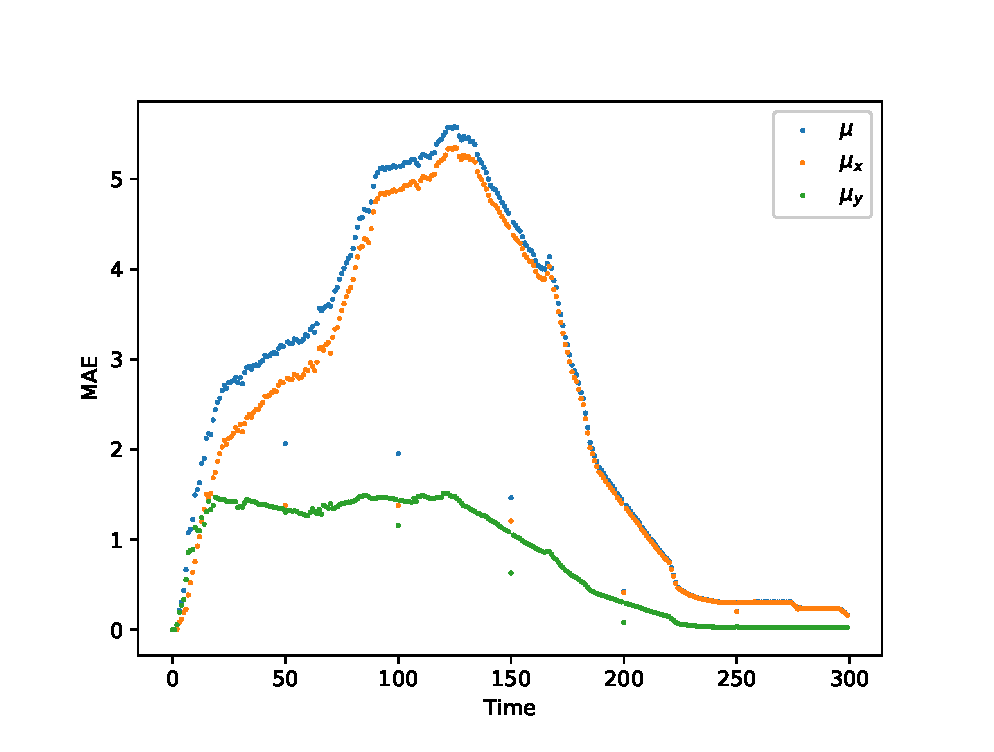
\includegraphics[width=0.8\textwidth]{errors}
    %\caption{Variation of errors with simulation time.}
    %\label{fig:errors}
%\end{figure}


\chapter{Conclusion}\label{ch:conclusion}

%This is the conclusion.
%\begin{itemize}
    %\item What does this investigation aim to do?
    %\item How does it do it?
    %\item Is is successful, and if so how successful?
    %\item What are the limitations?
%\end{itemize}

This investigation aimed to tackle the challenge of real-time simulation of
urban pedestrian systems.
It was identified that whilst much work existed on the use of agent-based models
to simulate such systems, the majority of these models were used as offline
tools that were calibrated before running but not updated with observations of
the system as they became available.
Given the stochastic nature of the models, this often results in model
states diverging from the real state of the system that they seek to simulate.
This issue owes largely to the lack of existing methods by which we can update
model states based on observational data without interrupting the model
progress.

One method that has been identified as a candidate to help resolve this issue is
data assimilation --- a group of techniques often used in the field of numerical
weather prediction.
In particular, this investigation focuses on the implementation of an Ensemble
Kalman Filter in conjunction with an agent-based model of pedestrians traversing
a rectangular station environment from entrances on one side to exits on the
opposite side.
This investigation aims to act as a proof-of-concept to demonstrate that the
Ensemble Kalman Filter can be used to improve the accuracy with which the model
simulates the true state of the system.
As such, the data assimilation method makes use of synthetic data generated by
the same agent-based model regarding the position of each of the agents.
The data is generated by adding normally distributed random noise to the ``true
state'', and is provided to the Ensemble Kalman Filter with a frequency
determined by the \emph{assimilation period}.

For the set of filter parameters and model parameters used (Tables
\ref{tab:filter_params} and \ref{tab:model_params}), the Ensemble Kalman Filter
was seen to improve the accuracy with which the model simulated the state of the
system.
This was examined on three levels.
Firstly we considered the agent positions in the model by taking the mean over
each of the ensemble member realisations, comparing the positions relative to
the true state before and after updating.
Secondly, we considered each of the individual realisations for a single agent,
comparing the positions relative to the true state before and after updating.
Finally we considered the root-mean-square error (where error is taken as
distance between mean agent position and true state position, and  averaging is
undertaken over each of the agents) and how it varies before and after updating
at each assimilation step.
In each case, the Ensemble Kalman Filter was seen to successfully improve the
accuracy with which the model simulated the system.

The investigation, however, is limited in a number of ways.
First and foremost, this investigation focuses exclusively on a single set of
model and filter parameters; the investigation has not explored the impact of
variation in model and filter parameters, and indeed whether the Ensemble Kalman
Filter is still effective for other parameter sets.

Beyond this, the investigation has assumed that the filter has perfect knowledge
of each agents' entrance and exit attributes at the beginning of the simulation
--- this would not typically be the case.
An agent's exit attribute, in particular, is of importance as it dictates the
direction in which the agent seeks to move.
Incorrect exit attributes for agents may therefore result in the model
persistently attempting to direct some agents to incorrect exits

%Problems to consider:
%\begin{itemize}
    %\item What happens when agents leave the system --- does the filter
        %recognise this correctly?
    %\item What happens when we are provided with aggregated information?
    %\item What happens when we are provided with different levels of information
        %for different agents?
    %\item Can the filter tell agents apart?
    %\item We have artificially told the filter information about agents'
        %entrance and exits - what happens if it doesn't know these? Do we then
        %need to do some assimilation for data assimilation?
%\end{itemize}

\section{Future Work}\label{sec:conc:future}

As noted above, the work presented herein is only a preliminary investigation
and consequently is limited.
The first avenue for future work would therefore be to expand on this
investigation by exploring the impact of each of the parameters provided to the
filter (as shown in Table \ref{tab:filter_params}).
Particular focus should be given to investigating the effects of varying the
assimilation period, the ensemble size and the observation error.
This may require the used of multithreading as the computational cost increases.
Care should be taken in implementing such an approach, however, as there may
come a point where the cost of passing information between threads outweighs the
benefit of splitting work between multiple processes.
%We would expect the following relationships to arise:
%\begin{itemize}
    %\item As the assimilation period is reduced, the error with which the model
        %simulates the system reduces; less model-time occurs between
        %observations being assimilated and consequently there is less time in
        %which the model can diverge from the ``true'' state.
    %\item As the ensemble size increases, the error with which the model
        %simulates the system reduces.
    %\item As the standard deviation of the observation error increases, the
        %Kalman gain matrix will likely bias in favour of the model state over
        %the observed state, and consequently the 
%\end{itemize}

Beyond this, attention should be given to the information provided to the data
assimilation method.
In this investigation, we have assumed that we have positional information about
each of the individual agents at each of the assimilation steps, however this is
seldom the case \citep{council2019leeds}.
The observations provided may be deficient in any of the following ways:
\begin{itemize}
    \item Observations only provided for a subset of the population.
    \item Observations provided for different agents at different assimilation
        steps.
    \item Observations provided in aggregated form. 
\end{itemize}
Each of these scenarios present different problems, each of which warrant
investigation.
Furthermore, it is assumed that the filtering method has knowledge of other
agent attributes such as their entrance and exits gates --- in reality, this is
unlikely to be the case.
Consequently, further investigations may seek to explore the impact of the
filter lacking this information, and the effect of trying to remedy the problem.
Such a solution might take the form of including parameters in the state vector
in order to also use data assimilation for parameter estimation.

%Ideas for transfer:
%\begin{itemize}
    %\item Explore impact of different filter parameters on filter performance
    %\item Explore impact of missing information; this can come in the form of
        %less frequent observation, observations of a selection of the agents.
    %\item Explore impact of aggregated observation
    %\item Include derivation of multivariate Kalman filter
    %\item Exploration of complexity of code (time and space)
    %\item Multithreading to deal with computational cost - identifying cut-off
        %point below which it is better to use serial computation. This doesn't
        %seem necessary at this stage as code runs in reasonable time with given
        %parameters, but something to consider for larger ensemble sizes,
        %population sizes. There will likely be some trade-off when looking at
        %assimilation period due to cost of message passing.
%\end{itemize}

The related data assimilation method known as the Particle Filter has also been
applied to the model presented in this investigation.
A further piece of work may aim to compare the efficacy of the two methods.
Whilst the main consideration such an investigation should be the effectiveness
with which each filter can reduce simulation error, some consideration should
also be given to a comparison of their computational complexity, i.e.\ the way
in which the time and memory required by the program scale with respect to
program parameters, with a view to exploring the trade-off of filter performance
and complexity.

Finally, it should also be noted that whilst this investigation made use of the
Ensemble Kalman filter, a number of variants of this method exist
\citep{keller2018comparing, katzfuss2016understanding} which aim to address
different problems that may be encountered.
Some of these may be of use when address further performance issues.

%Different types of EnKF and the implications for ensemble size
%\citep{keller2018comparing}.
%\begin{itemize}
    %\item Damping: counteract filter divergence
    %\item Localisation: reduce the effect of spurious correlations
    %\item Hybrid EnKF: Covariance matrix is made up of the weighted sum of the
        %usual covariance matrix and a separate static covariance matrix that
        %encodes prior underlying knowledge about the system
    %\item Dual EnKF: Split the state vector into state and parameters. At
        %assimilation: update parameters, recalculate forecast, update state
    %\item Normal Score EnKF: Developed to handle non-Gaussian PDFs in EnKF. At
        %assimilation: transform state, parameters and measurements into
        %Z-scores, perform EnKF update based on transformed values, transform
        %back from Z-scores
    %\item Iterative EnKF
%\end{itemize}

%Extensions to the EnKF \cite{katzfuss2016understanding}:
%\begin{itemize}
    %\item Variance inflation: often have ensemble size much smaller than state
        %dimension, which can mean that $\mathbf{K}$ can be a poor approximation
        %of the kalman gain matrix; we can therefore get downwardly biased
        %estimates of the posterior state covariance matrix ---  we can fix this
        %with covariance inflation whereby we multiply the covariance matrix by a
        %constant (greater than one). (Should check if this is an issue that we
        %need to consider).
    %\item Localisation: small ensemble sizes can result in spurious
        %correlations between state components that are physically far apart ---
        %we can use localisation to avoid this.
    %\item Parameter estimation: 
%\end{itemize}



\begin{appendix}
    %\appendix
\chapter{Code Documentation}\label{app:code_docs}

This is where I explain the design choices for how the enkf was coded.

\begin{itemize}
    \item options for generating observations:
        \begin{itemize}
            \item external
                \begin{itemize}
                    \item observations come from a previous model run as
                    synthetic data
                    \item therefore they should be independent
                    \item the problem here is that the ensemble members probably
                    have been set with the wrong entrances and exits or agents
                    \item this is likely more realistic, because when modelling
                    people we ultimately won't know where they intend to go
                    \item but we may be able to overcome this using parameter
                    estimation DA.
                \end{itemize}
            \item internal
                \begin{itemize}
                    \item observations come from the \texttt{base\_model}
                    \item all ensemble members are deep copies of the
                    \texttt{base\_model}
                    \item consequently, they have the same parameters and
                    initial conditions
                    \item problem here is that it's not very realistic
                    \item but we're going with it for this particular version
                \end{itemize}
        \end{itemize}
\end{itemize}


    \chapter{Bayes Rule}\label{ch:bayes}

The joint probability --- $P(A, B)$ --- is the probability of event $A$ occurring
and event $B$ occurring.
The conditional probability --- $P(A | B)$ --- is the probability of event $A$
occurring given that event $B$ occurs.
The joint and conditional probabilities are linked by the following relationship:
\begin{equation}
    P(A, B) = P(A) P(B | A).
\end{equation}
Similarly, we have
\begin{equation}
    P(B, A) = P(B) P(A | B).
\end{equation}
Given that the joint probabilities of $A, B$ and $B, A$ are equal:
\begin{equation*}
    P(A, B) = P(B, A),
\end{equation*}
we have that
\begin{equation}
    P(A) P(B | A) = P(B) P(A | B).
\end{equation}
From this, we can derive the typical form of Bayes Rule:
\begin{equation}
    P(B | A) = \frac{P(A | B) P(B)}{P(A)}
\end{equation}

\end{appendix}

\bibliographystyle{agsm}
\bibliography{references}

\end{document}
